\documentclass[a4paper,11pt]{article}

\usepackage{amsmath,amssymb,amsthm,amsopn,natbib,anysize}
\marginsize{2.5cm}{2.5cm}{2.5cm}{2.5cm}


\renewcommand{\today}{\begingroup
\number \day\space  \ifcase \month \or January\or February\or March\or 
April\or May\or June\or July\or August\or September\or October\or 
November\or December\fi 
\space  \number \year \endgroup}

\renewcommand{\vec}[1]{\boldsymbol{#1}}
\newcommand{\gvec}[1]{\boldsymbol{#1}}
\newcommand{\mat}[1]{\mathbf{#1}}
\newcommand{\gmat}[1]{\boldsymbol{#1}}
\newcommand{\bmat}[4]{\begin{bmatrix} #1 & #2 \\ #3 & #4\end{bmatrix}}
\newcommand{\argmin}[1]{\underset{#1}{\mathrm{argmin}} \ }
\newcommand{\argmax}[1]{\underset{#1}{\mathrm{argmax}} \ }
\newcommand{\indi}[1]{\boldsymbol{1} \lbrace #1 \rbrace}

\def\jneqi{\substack{j=1 \\ j\neq i}}
\def\kneqj{\substack{k=1 \\ k\neq j}}
\def\Hmat{\mat{H}}
\def\G{\mat{G}}
\def\ks{\texttt{ks}}
\def\sm{\texttt{sm}}
\def\KernSmooth{\texttt{KernSmooth}}
\def\MSE{\mathrm{MSE}}
\def\MISE{\mathrm{MISE}}
\def\AMSE{\mathrm{AMSE}}
\def\AMISE{\mathrm{AMISE}}
\def\SAMSE{\mathrm{SAMSE}}
\def\SCV{\mathrm{SCV}}
\def\PI{\mathrm{PI}}
\def\NR{\mathrm{NR}}
\def\BCV{\mathrm{BCV}}
\def\LSCV{\mathrm{LSCV}}
\def\MR{\mathrm{MR}}
\def\vecr{\vec{r}}
\def\vecx{\vec{x}}
\def\vecy{\vec{y}}
\def\vecX{\vec{X}}
\def\intr2{\int_{\boldsymbol{\mathbb{R}}^2}}
\def\intrd{\int_{\boldsymbol{\mathbb{R}}^d}}

\DeclareMathOperator{\E}{\boldsymbol{\mathbb{E}}}
\DeclareMathOperator{\Var}{Var}
\DeclareMathOperator{\Cov}{Cov}
\DeclareMathOperator{\Prob}{\boldsymbol{\mathbb{P}}}
\DeclareMathOperator{\given}{\vert}
\DeclareMathOperator{\Bias}{Bias}
\DeclareMathOperator{\VEC}{vec}
\DeclareMathOperator{\VECH}{vech}
\DeclareMathOperator{\tr}{tr}
\DeclareMathOperator{\dg}{dg}
\DeclareMathOperator{\diag}{diag}
\let\code=\texttt
\let\proglang=\texttt
\let\pkg=\texttt

%\VignetteIndexEntry{kde} 
%\SweaveOpts{eps=FALSE}

\title{ks: Kernel density estimation for bivariate data}
\author{Tarn Duong \\Department of Statistics, University of New South Wales\\ Sydney Australia}


\usepackage{/usr/share/R/share/texmf/Sweave}
\begin{document}

\maketitle


Kernel density estimation is a popular tool for visualising 
the distribution of data. See \citet*{simonoff1996}, for example, for
an overview.
When multivariate kernel density estimation is considered it is usually
in the constrained context with diagonal bandwidth matrices, e.g. 
in the \proglang{R} packages \pkg{sm} \citep*{sm} and \pkg{KernSmooth} 
\citep*{KernSmooth}.  
We introduce a new \proglang{R} package \pkg{ks} 
which implements diagonal and unconstrained data-driven bandwidth matrices
for kernel density estimation,
%The main theoretical advances underlying this package 
%are in the development of new methods for the latter for general dimensions.
which can also be used for multivariate kernel
discriminant analysis.  
The \pkg{ks} package implements selectors for  2- to 6-dimensional
data. 

This vignette contains only a brief introduction 
to using \pkg{ks} for kernel density estimation
for 2-dimensional data. 
See \citet*{duong2007c} for a more detailed account. 


For a bivariate random sample $\vecX_1, \vecX_2, \ldots, \vecX_n$ 
drawn from a density $f$, 
the kernel density estimate is defined by
$$
\hat{f} (\vecx; \Hmat) = n^{-1}\sum_{i=1}^n K_{\Hmat} ( \vecx - \vec{X}_i)
$$
where $\vecx = (x_1, x_2)^T$ and $\vec{X}_i = (X_{i1}, X_{i2})^T, i = 1, 2,  
\ldots, n$.  Here 
$K(\vecx)$ is the kernel which is a symmetric probability density function, 
$\Hmat$ 
is the bandwidth matrix which is symmetric and positive-definite,  
and $K_{\Hmat}(\vecx) = |\Hmat|^{-1/2} 
K( \Hmat^{-1/2} \vecx)$. 
The choice of $K$ is not crucial: we take 
$K(\vecx) = (2\pi)^{-1} \exp(-\tfrac{1}{2} \vecx^T \vecx)$ the standard normal
throughout.  
In contrast, the choice of $\Hmat$ is crucial in determining 
the performance of $\hat f$. 
The most common parameterisations of the bandwidth matrix
are the diagonal and the 
general or unconstrained which has no restrictions on $\Hmat$
provided that $\Hmat$
remains positive definite and symmetric, that is 
$$
\Hmat = \begin{bmatrix}h_1^2 & 0 \\0 & h_2^2 \end{bmatrix}
\ \mathrm{or} \ 
\Hmat = \begin{bmatrix}h_1^2 & h_{12} \\ h_{12}  & h_2^2 \end{bmatrix}.
$$
This latter
parameterisation allows kernels to have an arbitrary orientation
whereas the former only allows kernels which are oriented to the
co-ordinate axes.

For our target density, we use the 
 `dumbbell' density, given by the normal mixture
$$ \frac{4}{11} N \bigg( \begin{bmatrix}-2 \\ 2\end{bmatrix}, 
\begin{bmatrix}1 & 0 \\ 0 & 1 \end{bmatrix} \bigg)+ 
\frac{3}{11} N \bigg( \begin{bmatrix}0 \\ 0\end{bmatrix},
\begin{bmatrix}0.8 & -0.72 \\ -0.72 & 0.8\end{bmatrix} \bigg)+
\frac{4}{11} N \bigg( \begin{bmatrix}2 \\ -2\end{bmatrix}, 
\begin{bmatrix}1 & 0 \\ 0 & 1 \end{bmatrix} \bigg),
$$
displayed on the left in Figure \ref{fig:dens-db}. This 
density is unimodal. On the right is a
sample of 200 data points.
 
\begin{Schunk}
\begin{Sinput}
> library(ks)
> set.seed(8192)
> samp <- 200
> mus <- rbind(c(-2, 2), c(0, 0), c(2, -2))
> Sigmas <- rbind(diag(2), matrix(c(0.8, -0.72, -0.72, 0.8), nrow = 2), 
+     diag(2))
> cwt <- 3/11
> props <- c((1 - cwt)/2, cwt, (1 - cwt)/2)
> x <- rmvnorm.mixt(n = samp, mu = mus, Sigma = Sigmas, props = props)
\end{Sinput}
\end{Schunk}

\setkeys{Gin}{width=0.45\textwidth}
\begin{figure}[!ht]
\begin{center}
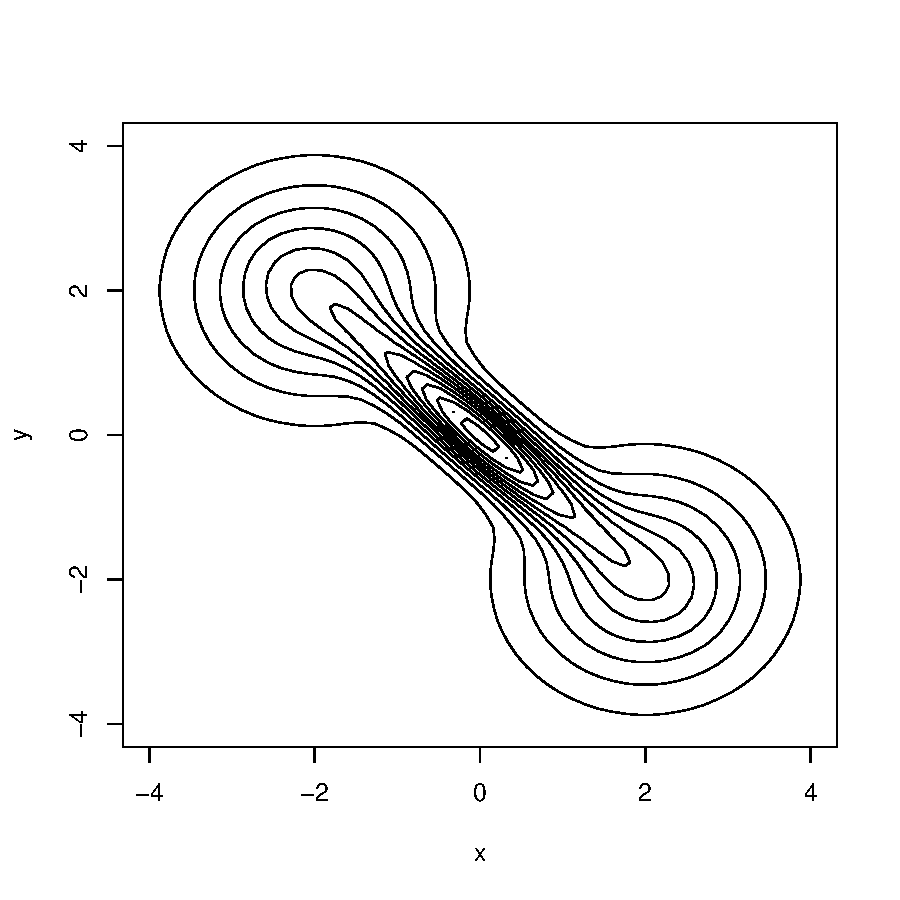
\includegraphics{kde-002}
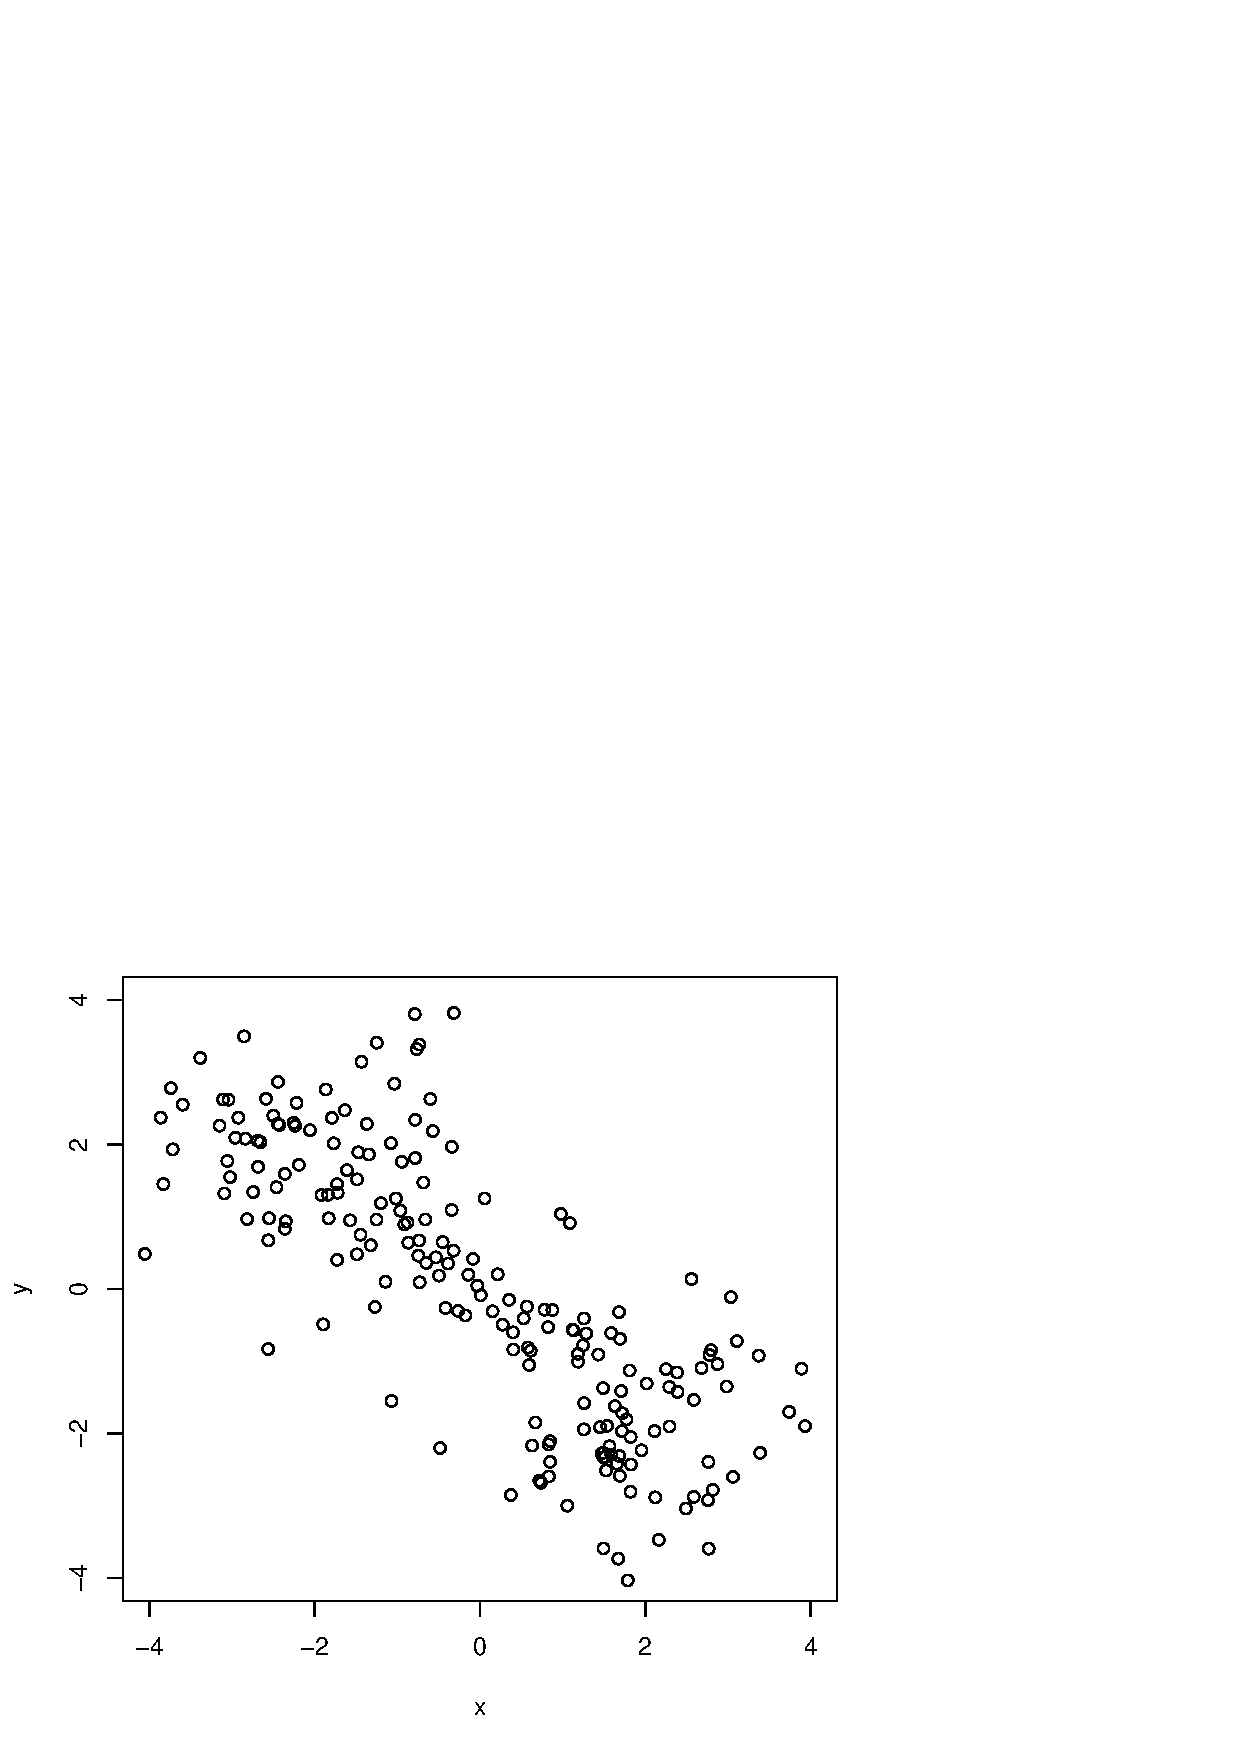
\includegraphics{kde-003}
\end{center}
\caption{Target `dumbbell' density. (Left) contour plot. (Right) Scatter plot.}
\label{fig:dens-db}
\end{figure}



We use \code{Hpi} for 
unconstrained plug-in selectors and \code{Hpi.diag} for diagonal plug-in selectors.
\begin{Schunk}
\begin{Sinput}
> Hpi1 <- Hpi(x = x)
\end{Sinput}
\begin{Soutput}
           [,1]       [,2]
[1,]  0.4054542 -0.2778998
[2,] -0.2778998  0.3349442
\end{Soutput}
\begin{Sinput}
> Hpi2 <- Hpi.diag(x = x)
\end{Sinput}
\begin{Soutput}
          [,1]      [,2]
[1,] 0.1859013 0.0000000
[2,] 0.0000000 0.1312804
\end{Soutput}
\end{Schunk}
To compute a kernel density estimate, the 
command is \code{kde}, which creates a \code{kde} class object
\begin{Schunk}
\begin{Sinput}
> fhat.pi1 <- kde(x = x, H = Hpi1)
> fhat.pi2 <- kde(x = x, H = Hpi2)
\end{Sinput}
\end{Schunk}
We use the \code{plot} method for \code{kde} objects to display these
kernel density estimates. The default is a contour plot with 
the upper 25\%, 50\% and 75\% contours of the 
(sample) highest density regions. %, as
%defined in \citet*{bowman1993} and \citet*{hyndman1996}.
These regions are also plotted by the \pkg{sm} library.
\begin{Schunk}
\begin{Sinput}
> plot(fhat.pi1)
> plot(fhat.pi2)
\end{Sinput}
\end{Schunk}
The respective kernel density estimates are produced in Figure \ref{fig:pi}.
The diagonal bandwidth matrix constrains the smoothing to be performed in directions
parallel to the co-ordinate axes, so it is not able to apply accurate levels
of smoothing to the obliquely oriented central portion. The result is a 
multimodal
density estimate. The unconstrained bandwidth matrix correctly produces 
a unimodal density estimate. 


\begin{figure}[!ht]
\centering
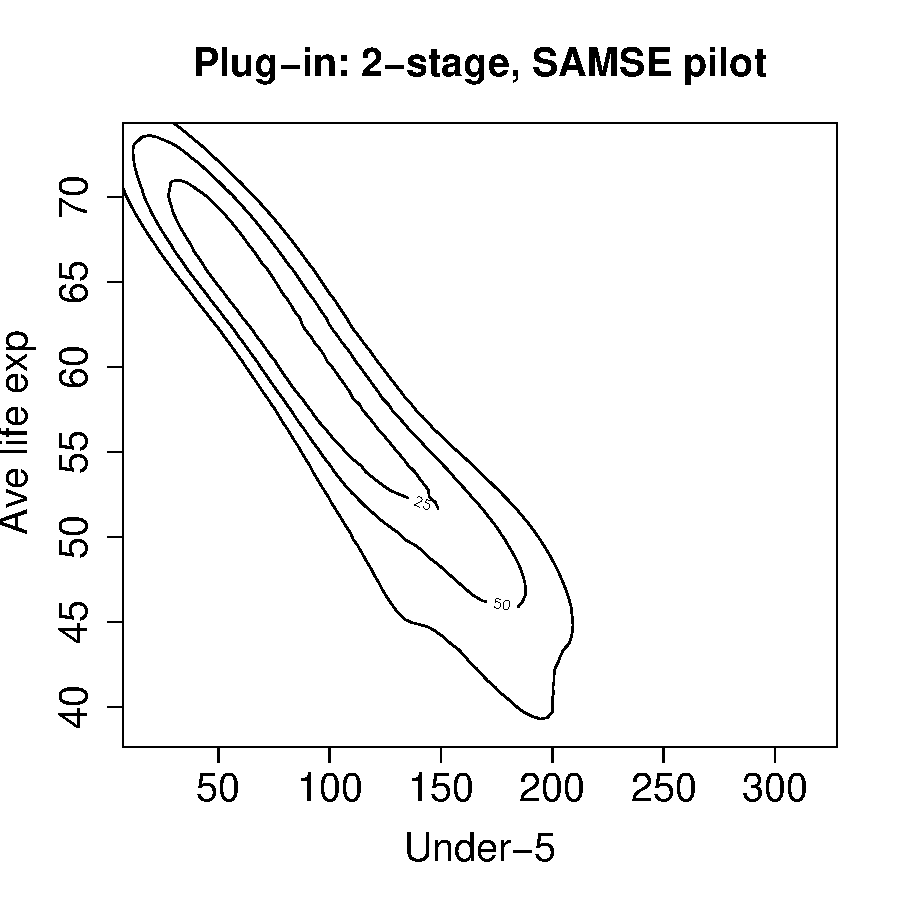
\includegraphics{kde-007}
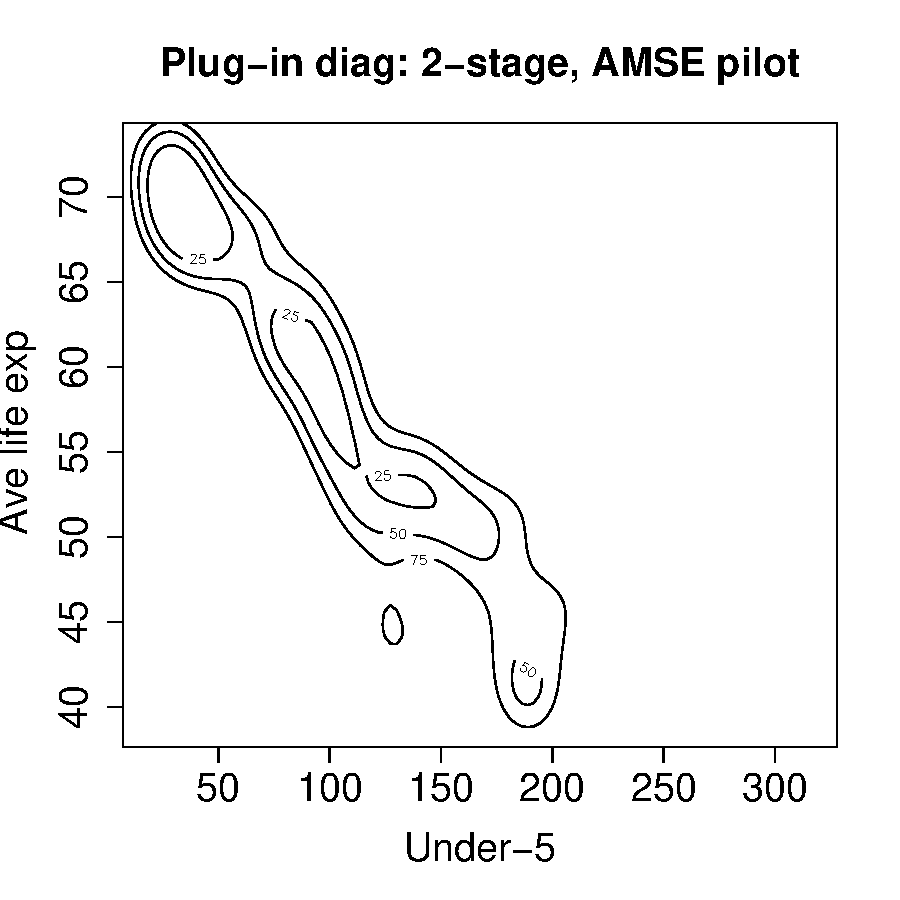
\includegraphics{kde-008}
\caption{Kernel density estimates with plug-in selectors}
\label{fig:pi}
\end{figure}


%The commands
%\code{Hlscv} and \code{Hlscv.diag} are the unconstrained and diagonal
%LSCV (Least Squares Cross Validation) selectors. 
The unconstrained SCV (Smoothed Cross Validation) selector is \code{Hscv} and 
its diagonal version is \code{Hscv.diag}.
In Figure \ref{fig:cv}, the most
reasonable density estimate is from the unconstrained SCV selector. 
 
\begin{Schunk}
\begin{Sinput}
> Hscv1 <- Hscv(x = x)
\end{Sinput}
\begin{Soutput}
           [,1]       [,2]
[1,]  0.5647800 -0.4044703
[2,] -0.4044703  0.4934641
\end{Soutput}
\begin{Sinput}
> Hscv2 <- Hscv.diag(x = x)
\end{Sinput}
\begin{Soutput}
         [,1]      [,2]
[1,] 0.284455 0.0000000
[2,] 0.000000 0.2460504
\end{Soutput}
\end{Schunk}

\begin{figure}[!ht]
\centering
\includegraphics{kde-011}
\includegraphics{kde-012}
%\includegraphics[height=6.8cm,width=6.8cm]{figures/db-cv1}
%\includegraphics[height=6.8cm,width=6.8cm]{figures/db-cv2} \\
%\includegraphics[height=6.8cm,width=6.8cm]{figures/db-cv3}
%\includegraphics[height=6.8cm,width=6.8cm]{figures/db-cv4} \\
%\includegraphics[height=6.8cm,width=6.8cm]{figures/db-cv5}
%\includegraphics[height=6.8cm,width=6.8cm]{figures/db-cv6}
\caption{Kernel density estimates with cross validation selectors}
\label{fig:cv}
\end{figure}


%So far the calls to \code{kde} compute $\hat{f}$ exactly. This exact 
%computation is $O(n^2)$ complexity which becomes infeasible for large
%sample sizes, say $n=10\ 000$ on a current desktop PC. 
% One common technique for increasing computational
%speed for these large samples is binned kernel estimation, 
%%see \citet*[Appendix~D]{wand1994} 
%as implemented in
%\pkg{KernSmooth} \citep*{KernSmooth}. 
%Binning converts the data sample of size $n$ to a grid of size $m$,
%so binned estimation remains $O(m)$ regardless of the sample size.
%A suitable binning grid size for bivariate data is $m = 151^2$.


%Binned estimation is only defined 
%with diagonal bandwidth matrices. Applicable cases include 
%kernel density estimators with diagonal bandwidth matrices and
%the pilot estimators for the plug-in and SCV selectors. 
%In the \code{Hpi}, \code{Hpi.diag}, \code{Hscv}, \code{Hscv.diag}
%and \code{kde} commands, we set \code{binned=TRUE}, e.g. 





%\section{General recommendations}
%\label{sec:rec}
%The different bandwidth selectors available in \pkg{ks} may
%now pose a problem of too much choice.
The unconstrained bandwidth selectors will be better than their diagonal counterparts
when the data have large mass oriented obliquely to the co-ordinate axes,
like for the dumbbell data. 
%Amongst the unconstrained selectors, %we advise against using the BCV selector. 
%The LSCV selector is useful in some cases though its performance is 
%known to be highly variable. 
The unconstrained plug-in and the SCV selectors
can be viewed as generally recommended selectors.



\bibliographystyle{apalike}

\begin{thebibliography}{}


\bibitem[Duong, 2007]{duong2007c}
Duong, T. (2007).
\newblock ks: {K}ernel density estimation and kernel discriminant analysis for
  multivariate data in {R}.
\newblock {\em Journal of Statistical Software}. In press.


\bibitem[Simonoff, 1996]{simonoff1996}
Simonoff, J.~S. (1996).
\newblock {\em Smoothing Methods in Statistics}.
\newblock Springer-Verlag, New York.

\end{thebibliography}

\end{document}



